% \documentclass{cmspaper}
%\begin{document}

\section{Electron Studies} \label{sec:electrons}

\subsection{Identification and Isolation} \label{sec:IdAndIso}

A reconstructed electron object is formed from deposition of energy in ECAL (called a ``supercluster'') that has an 
extrapolated track pointing to it.
This study uses the standard ``PixelMatchGsfElectrons'' collection of MC events\cite{GSFele}.
The reconstruction algorithm of Ref \cite{GSFele} first matches the supercluster to hits in the pixel detector.
The pixel hits are then used to seed a track.  Finally, a track is fit to all hits using the Gaussian Sum Filter 
(GSF) algorithm, which reconstructs the track to the ECAL surface
despite the possible presence of kinks from electron bremsstrahlung.  
The $p_{T}$ and $\eta$ of the electrons are calculated using both calorimeter and tracker information, 
taking account of detector resolutions and its dependence on $p_{T}$.
Standard CMS Software corrections are applied to set correctly the electromagnetic (EM) energy scale.

%#######Ref for CMSSW electron energy scale #############

%that is matched with hits in the pixel detector.  Few electrons loose momentum to radiated photons before the pixel detector since the majority of the material in the tracker is after the pixels.  Thus, the energy-weighted average impact point of the electrons and radiated photons with the supercluster will correspond well with the track found using these pixel hits as seeds.  

The criteria used for electron identification (ID) at the reconstruction level are very loose, thereby contributing many false electrons 
to the collection. In this analysis, the HEEP selections for electron ID and isolation \cite{EleID}, which are optimized for 
electrons with energies of hundreds of GeV, have been applied in an effort to: i) keep the efficiency high for electrons from LQ decays that have high $p_{T}$, and 
ii) reduce the number of jets mimicking electrons.
The definitions of the variables used in this analysis are given below:
%
\begin{itemize}
%
\item $H/E$: the ratio of the hadronic energy of all the highest HCAL Rec Hit to the electromagnetic energy of the supercluster associated with the electron.
%
\item $\sigma_{\eta\eta}$: a variable reflecting the longitudinal distribution of the electron shower (along $\eta$):
\begin{displaymath}
\sigma_{\eta\eta} = \sum( \eta_i - \eta_s )^2 \frac{E_i}{E_{\mbox{s}}} \quad ,
\end{displaymath}
where $E_i$ is the energy in the $i^(th)$ crystal, and $E_s$ is the the energy in the seed cluster of the electron's supercluster.
%
\item $\Delta\eta_{in}$ and $\Delta\phi_{in}$: the difference in $\eta$ and $\phi$ between the track position extrapolated from 
the inner layer tracker to the ECAL surface and the $\eta$ and $\phi$ of the supercluster.
%
\item Number of Tracks ($N_T$): with $p_{T}>1.5$ GeV in an annulus $0.1 < \Delta\mbox{R} < 0.2 $ around the direction of the electron;
%
\item Track Isolation (Track Iso): the sum of the $p_{T}$ of tracks (defined above) divided by the $E_{T}$ of the supercluster.

%############????????################

%
\item EM Isolation (Iso): the transverse part of the electromagnetic energy deposited in all the clusters in a cone $\Delta\mbox{R} < 0.3$, 
centered on the electron's position in the calorimeter, excluding the clusters that make up the supercluster;
%
\item HAD Isolation: the transverse part of the hadronic energy of all the HCAL Rec Hits with an $E_{T}>0$ in an annulus
$0.15 < \Delta\mbox{R} < 0.3$, centered on the electron's position in the calorimeter. 
%
\end{itemize}

Figures~\ref{fig:elecID} and ~\ref{fig:elecIso} show, respectively, distributions in ID and Isolation variables, 
for both true electrons from LQ decays and fake electrons from a sample of QCD multi jet events. 
Table~3
%\ref{tab:HEEPselection} 
summarizes the HEEPs selection used in this analysis. In addition, only reconstructed electrons with 
$p_{T}>30$ GeV and 
within the ECAL fiducial region 
$|\eta|<1.4$ + $1.6<|\eta|<2.0$ are included in the electron collection used in our analysis.  

Recentely HEEP EM and HAD Isolation criteria have been improved, 
leading to a better rejection of jets mimicking electrons, while keeping the same efficiency on true electrons.
The impact of this improvement will be investigated in 
future upgrades of this analysis. 

%The quantities used in this definition are the ratio of hadronic to electromagnetic energy (H/E), shower shape along psudorapidity ($\sigma_{\eta\eta}$), difference in psudorapidity between the track and the supercluster ($\Delta\eta_{in}$), and the difference in phi between the track and supercluster ($\Delta\phi_{in}$). These cuts are appropriate for start up conditions as they allow a high efficiency.  The quatities and values used for these selection can be found in table~\ref{tab:ElecIdIso}. Figure~\ref{fig:elecID} shows the distributions of these variables for both true electrons coming from the leptoquark decays and fake electrons from a QCD sample.

%Further cleaning of the collection is achieved through requiring that the electron be isolated.  The three quantities considered are the number of tracks within a cone of radius 0.2 of the contact with the supercluster, the ratio of the sum of transverse energy of tracks within a cone of radius 0.2 to that of the electron track (Track Et ratio), and the ratio of transverse energy in the ECAL within a cone of radius 0.4 to that of the electron (ECAL Et ratio).  These are also found in table~\ref{tab:ElecIdIso}.  The distributions of these variables for both true electrons from the leptoquark decay and fake electrons from QCD events can be seen in figure~\ref{fig:elecIso}
 
%From : twiki.cern.ch/twiki/bin/view/CMS/SWGuideEgamma

% Robust Electron Def from : twiki.cern.ch/twiki/bin/view/CMS/SWGuideElectronID
% Ele Isolation from : twiki.cern.ch/twiki/bin/view/CMS/SWGuideEgamma 

%Still need description of these plots, like what cuts were used...

%\begin{2figures}{hbtp}
%  \resizebox{\linewidth}{!}{\includegraphics{plots/h_eleDeltaEtaTrkSC.eps}} &
%  \resizebox{\linewidth}{!}{\includegraphics{plots/h_eleDeltaPhiTrkSC.eps}} \\
%  \caption{eleDeltaEtaTrkSC}
%  \label{fig:eleDeltaEtaTrkSC} &
%  \caption{\small \sl eleDeltaPhiTrkSC}
%  \label{fig:eleDeltaPhiTrkSC} \\
%\end{2figures}
%\begin{2figures}{hbtp}
%  \resizebox{\linewidth}{!}{\includegraphics{plots/h_eleHoE.eps}} &
%  \resizebox{\linewidth}{!}{\includegraphics{plots/h_eleSigmaEE.eps}} \\
%  \caption{\small \sl eleHoE}
%  \label{fig:eleHoE} &
%  \caption{\small \sl eleSigmaEE}
%  \label{fig:eleSigmaEE} \\
%\end{2figures}
%\begin{2figures}{hbtp}
%  \resizebox{\linewidth}{!}{\includegraphics{plots/h_eleNumTrkIso.eps}} &
%  \resizebox{\linewidth}{!}{\includegraphics{plots/h_eleEcalIso.eps}} \\
%  \caption{\small \sl eleNumTrkIso}
%  \label{fig:eleNumTrkIso} &
%  \caption{\small \sl eleEcalIso}
%  \label{fig:eleEcalIso} \\
%\end{2figures}
%\begin{figure}
%  \begin{center}
%    \resizebox{0.5\linewidth}{!}{\includegraphics{plots/h_eleTrkIso.eps}}
%    \caption{\small \sl eleTrkIso}
%    \label{fig:eleTrkIso}
%  \end{center}
%\end{figure}

\begin{figure}
  \begin{center}
  \begin{tabular}{cc}
  \resizebox{7cm}{!}{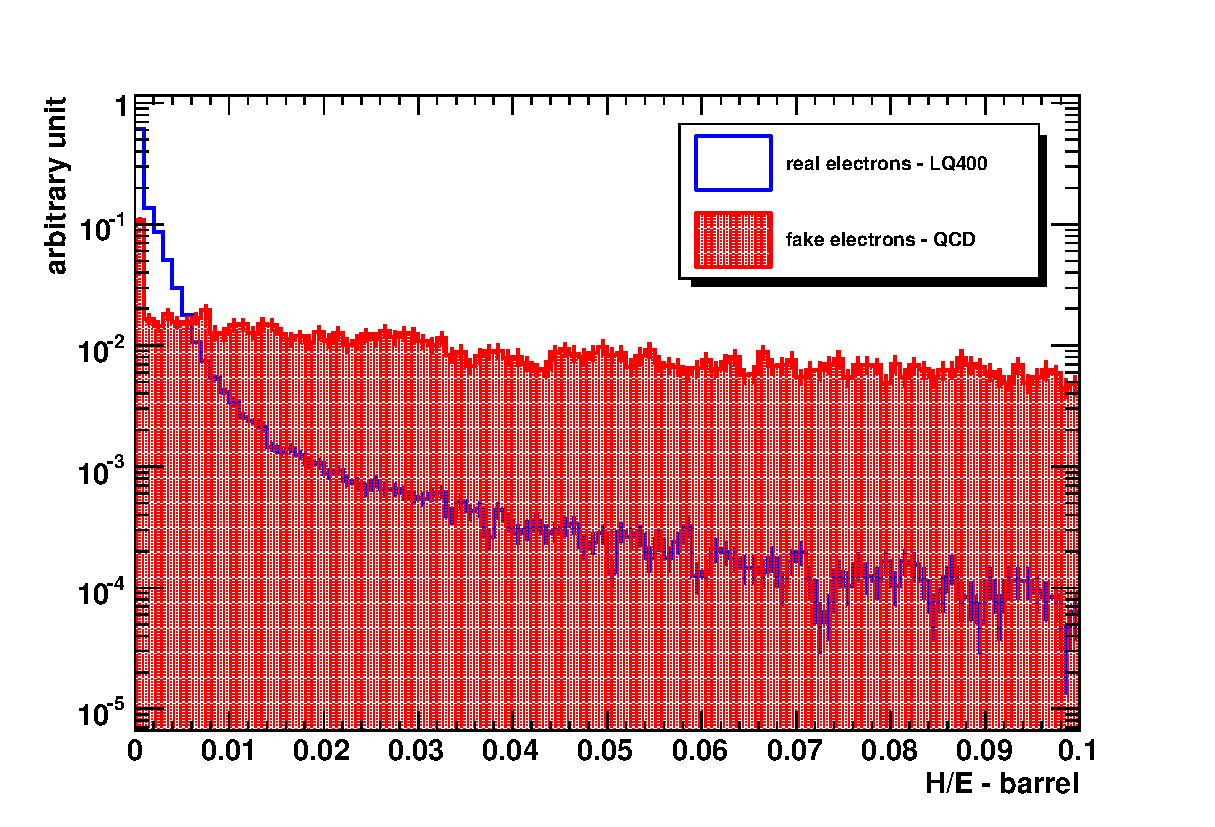
\includegraphics{plots/electronStudies/eleHoE_barrel_LQ400vsQCD.eps}} &
  \resizebox{7cm}{!}{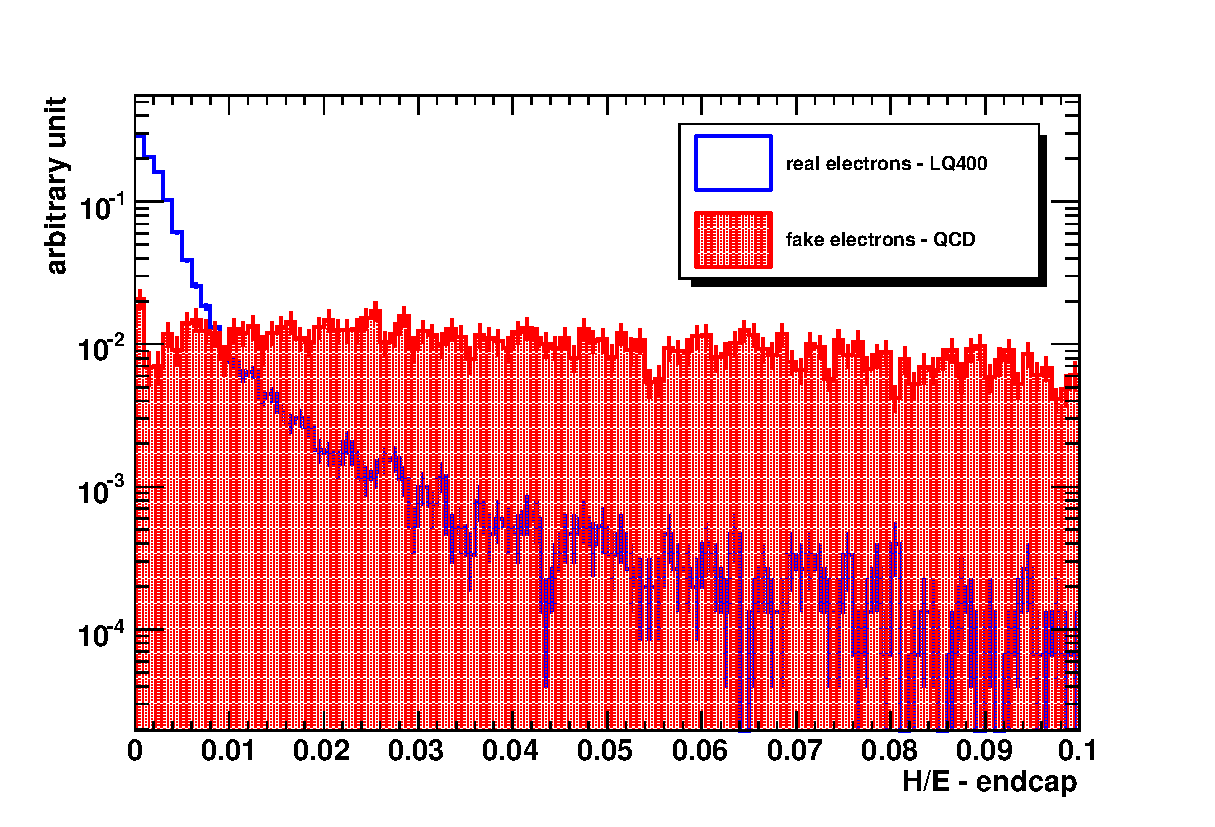
\includegraphics{plots/electronStudies/eleHoE_endcap_LQ400vsQCD.eps}} \\
  \resizebox{7cm}{!}{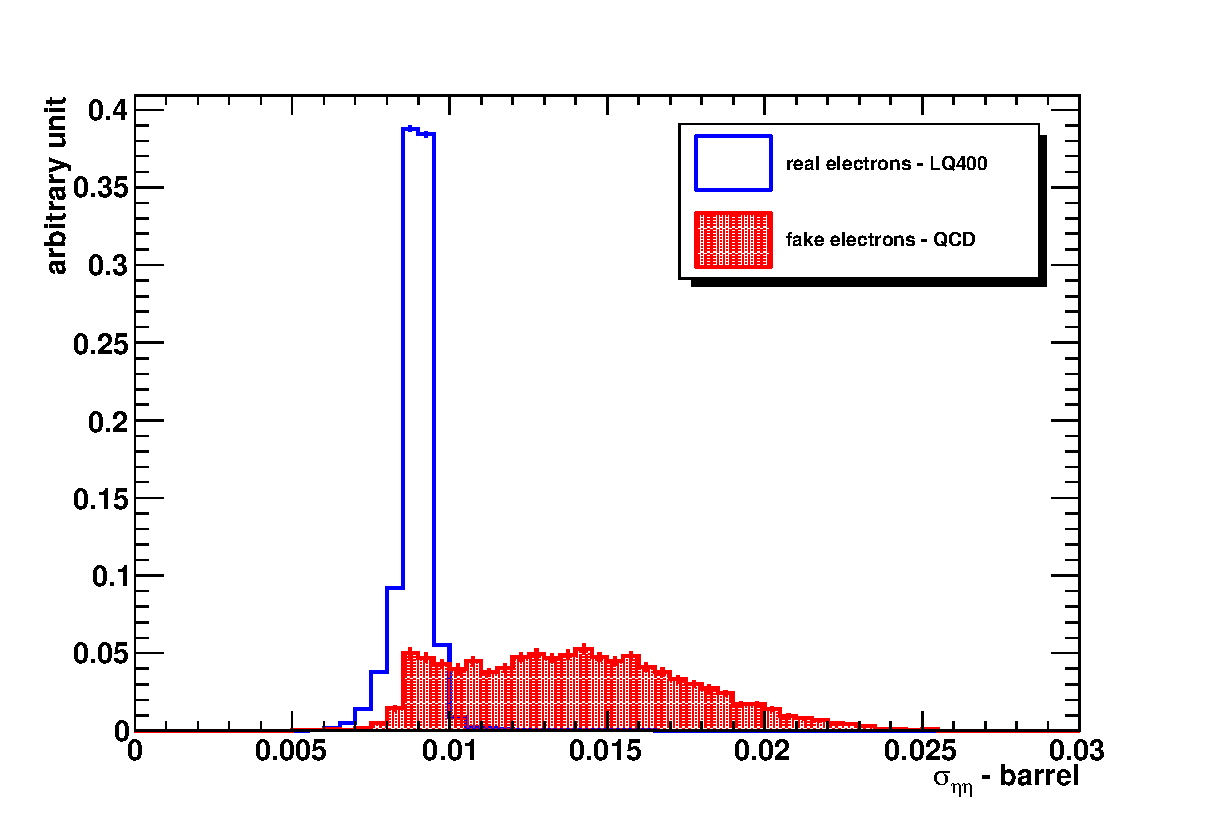
\includegraphics{plots/electronStudies/eleSigmaEE_barrel_LQ400vsQCD.eps}} &
  \resizebox{7cm}{!}{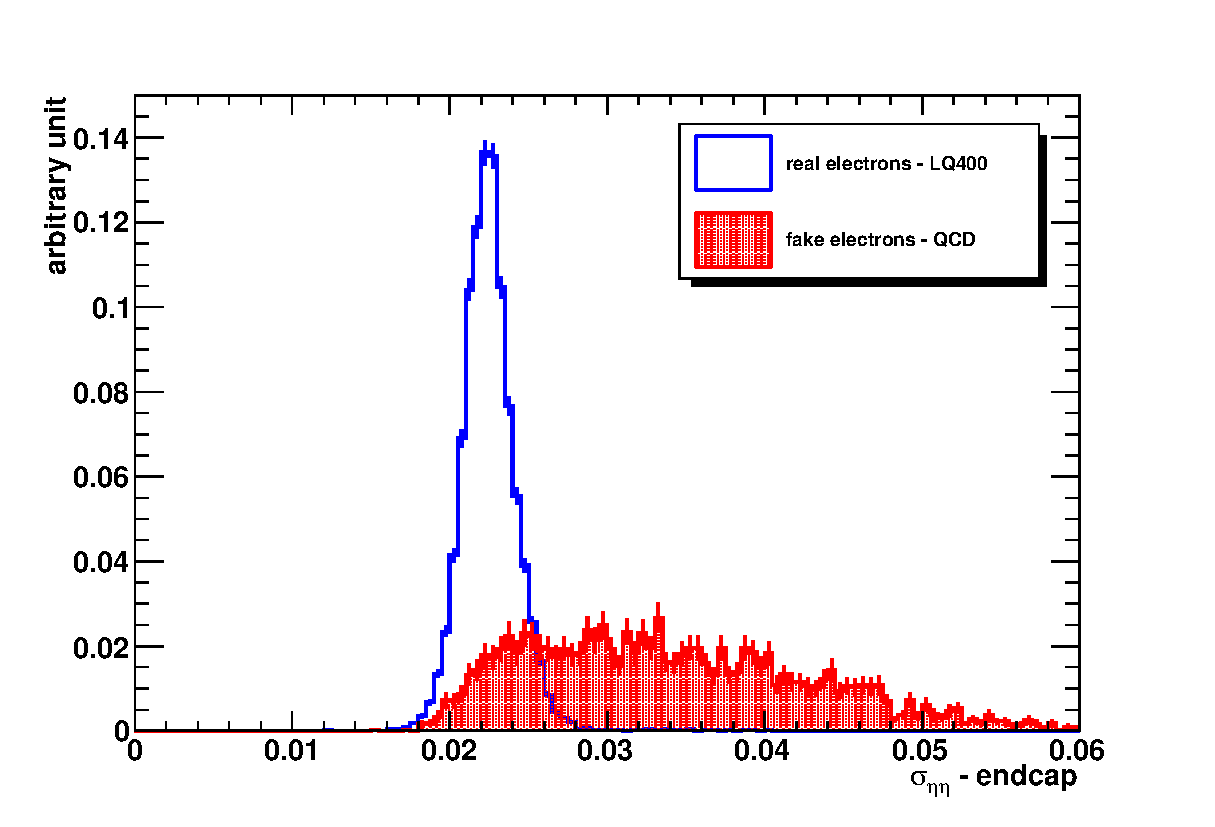
\includegraphics{plots/electronStudies/eleSigmaEE_endcap_LQ400vsQCD.eps}} \\
  \resizebox{7cm}{!}{\includegraphics{plots/electronStudies/eleDeltaEtaTrkSC_barrel_LQ400vsQCD.eps}} &
  \resizebox{7cm}{!}{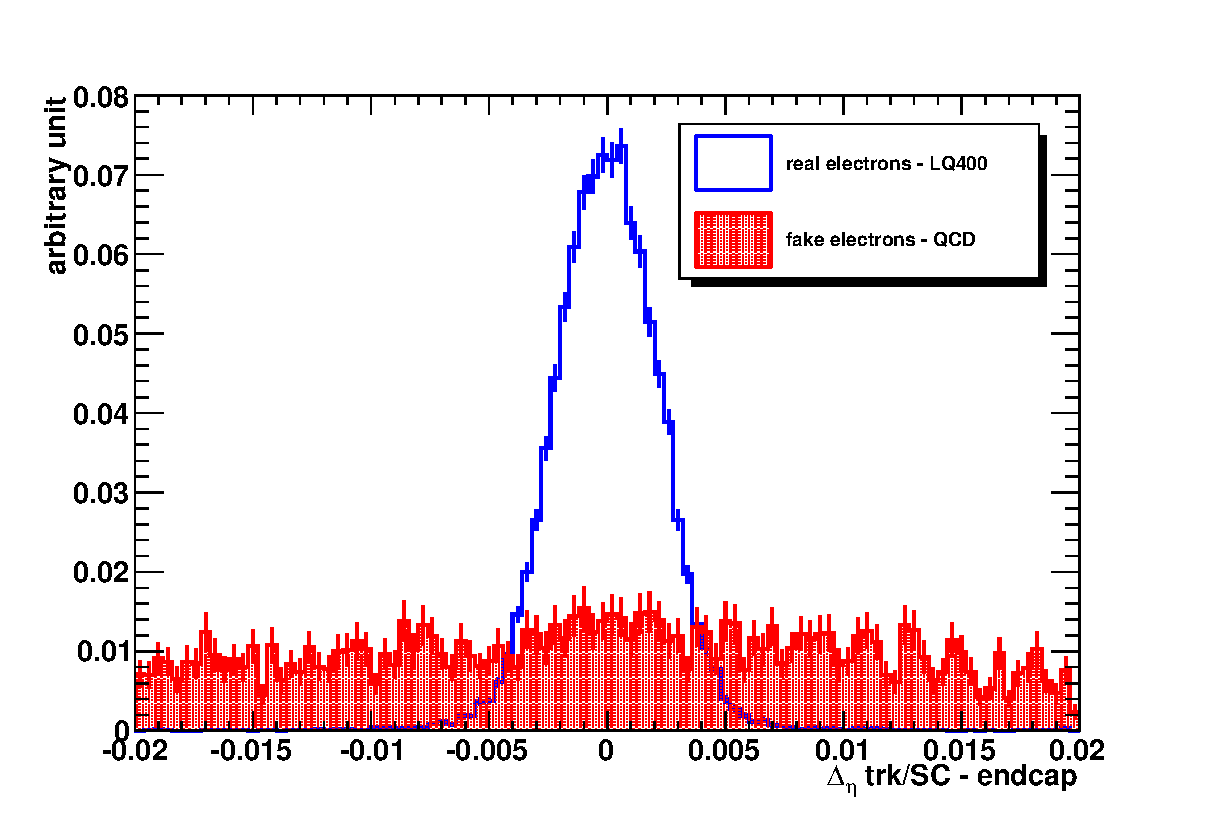
\includegraphics{plots/electronStudies/eleDeltaEtaTrkSC_endcap_LQ400vsQCD.eps}} \\
  \resizebox{7cm}{!}{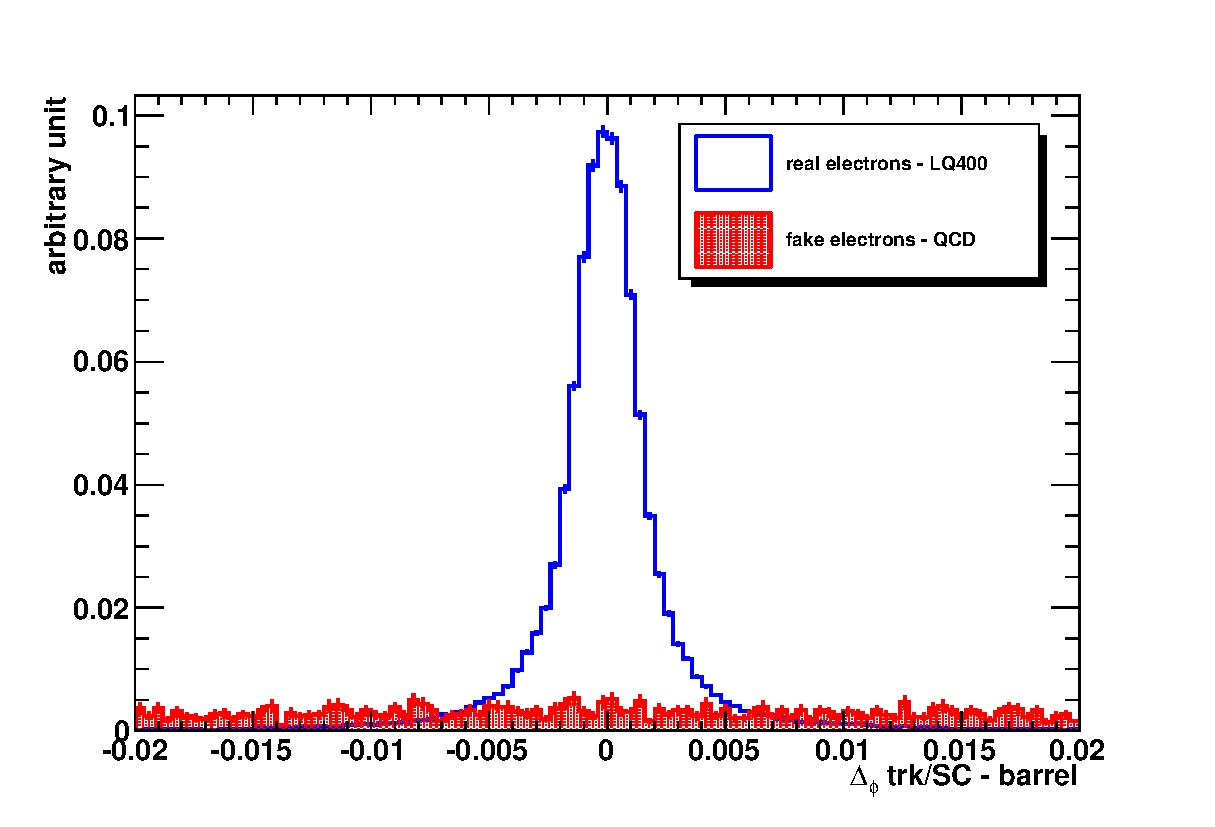
\includegraphics{plots/electronStudies/eleDeltaPhiTrkSC_barrel_LQ400vsQCD.eps}} &
  \resizebox{7cm}{!}{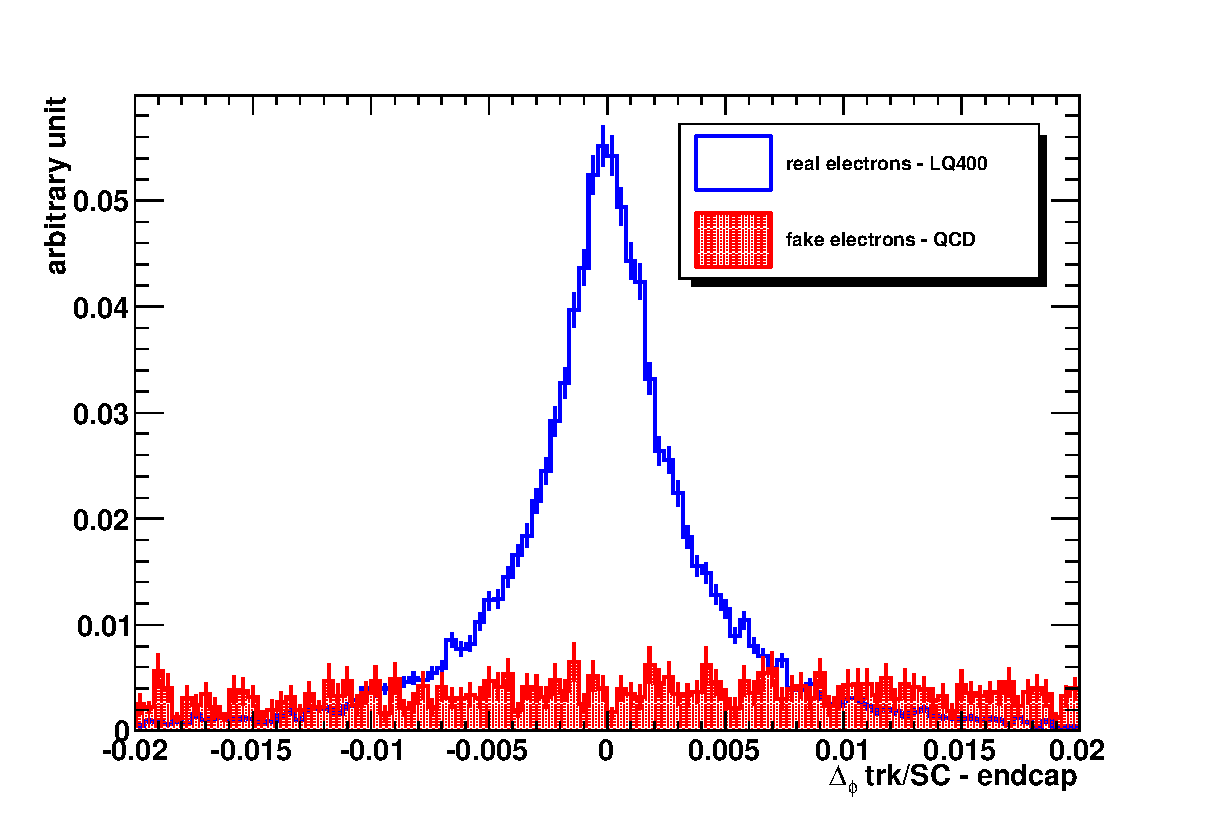
\includegraphics{plots/electronStudies/eleDeltaPhiTrkSC_endcap_LQ400vsQCD.eps}} \\
  \end{tabular} 
  \caption{\small \sl Distribution of electron-ID variables for true electrons from the decay of 400 GeV mass LQ, and false electrons from 
 QCD multi jets MC events. Electrons with $p_{T}>150$ GeV are made to undergo MC showering. ?????? FIXME. 
 Electrons from LQ decay are matched with reconstructed electrons if $\Delta$R between them is < 0.02. }
 \label{fig:elecID}
  \end{center}
\end{figure}

\begin{figure}
  \begin{center}
  \begin{tabular}{cc}
  \resizebox{7cm}{!}{\includegraphics{plots/electronStudies/eleNumTrkIso_barrel_LQ400vsQCD.eps}} &
  \resizebox{7cm}{!}{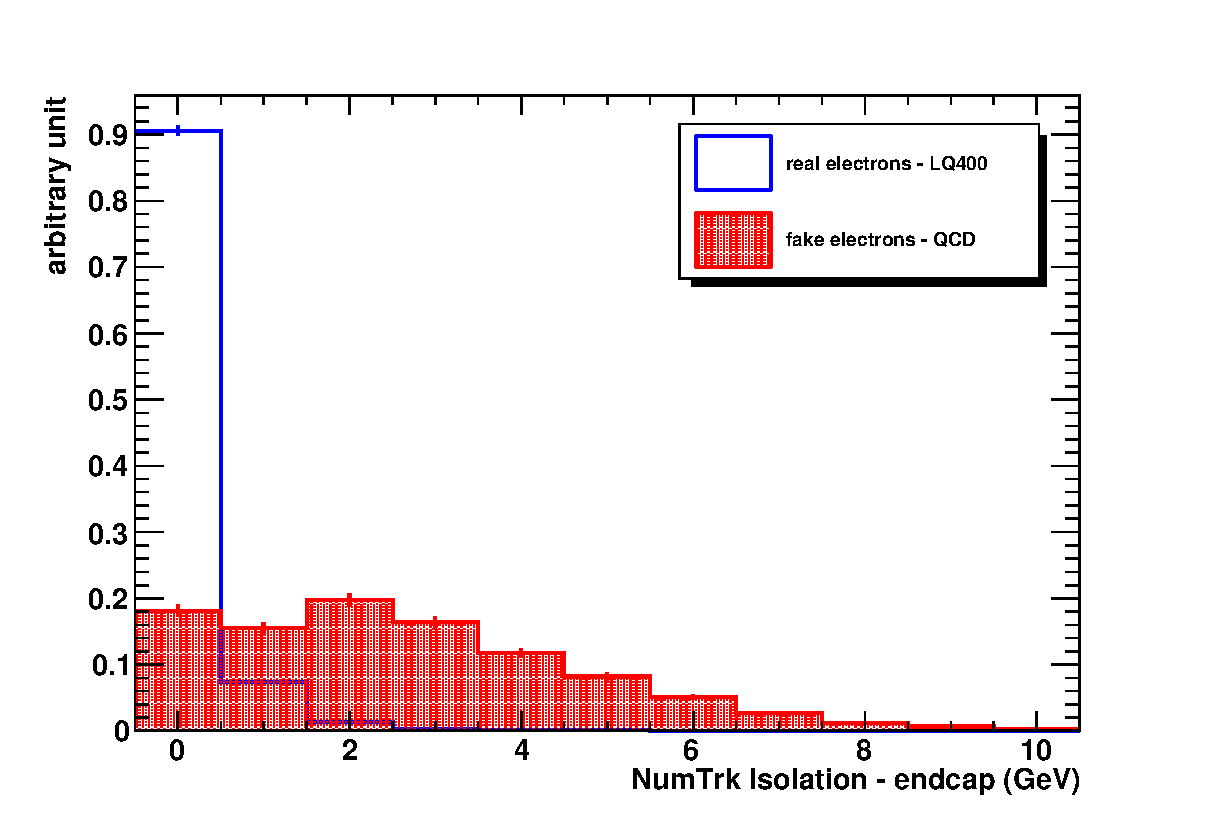
\includegraphics{plots/electronStudies/eleNumTrkIso_endcap_LQ400vsQCD.eps}}\\
  \resizebox{7cm}{!}{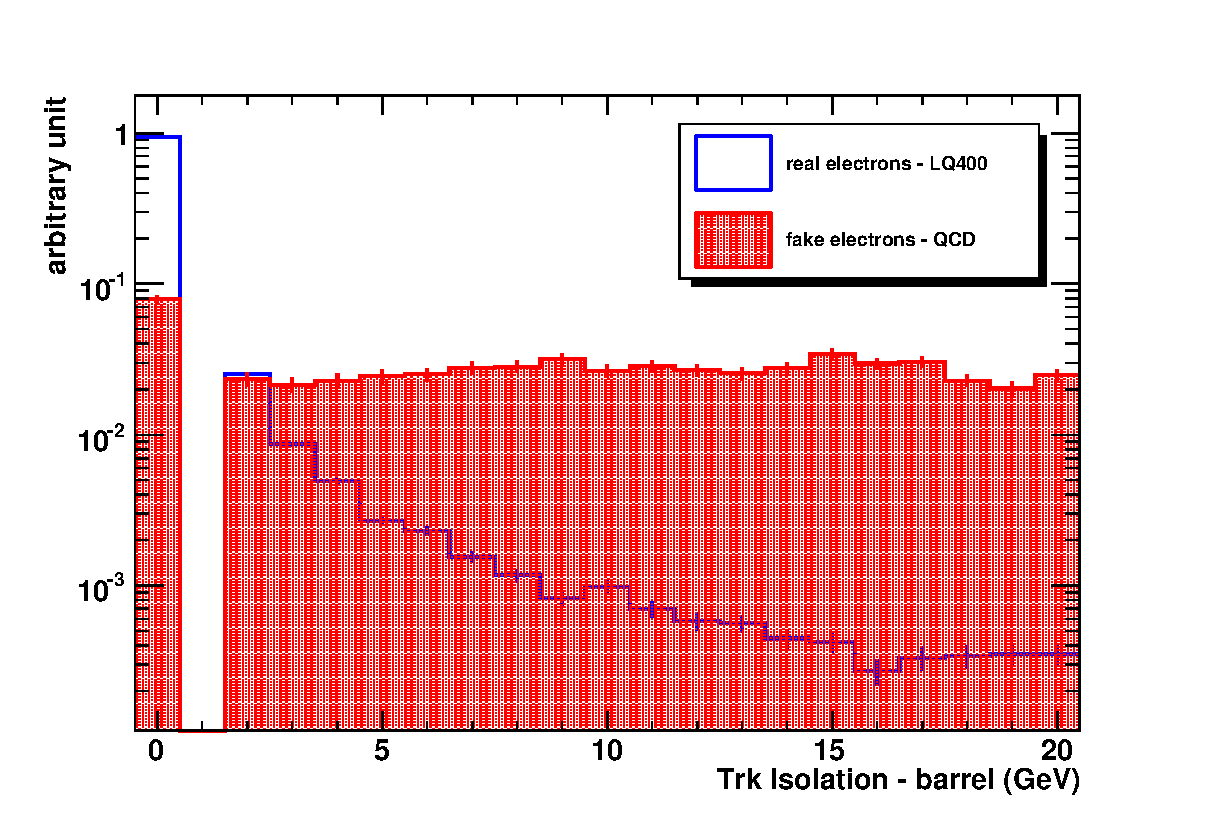
\includegraphics{plots/electronStudies/eleTrkIso_barrel_LQ400vsQCD.eps}} &
  \resizebox{7cm}{!}{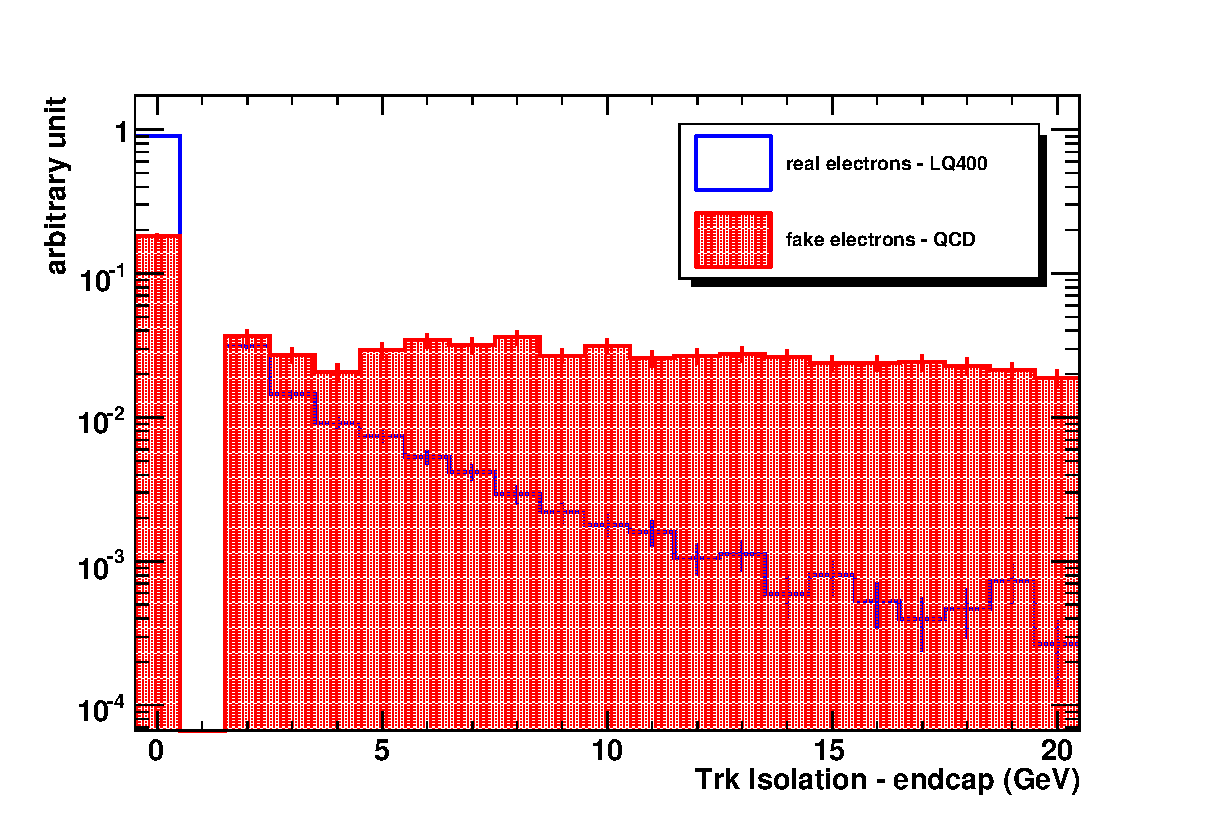
\includegraphics{plots/electronStudies/eleTrkIso_endcap_LQ400vsQCD.eps}} \\
  \resizebox{7cm}{!}{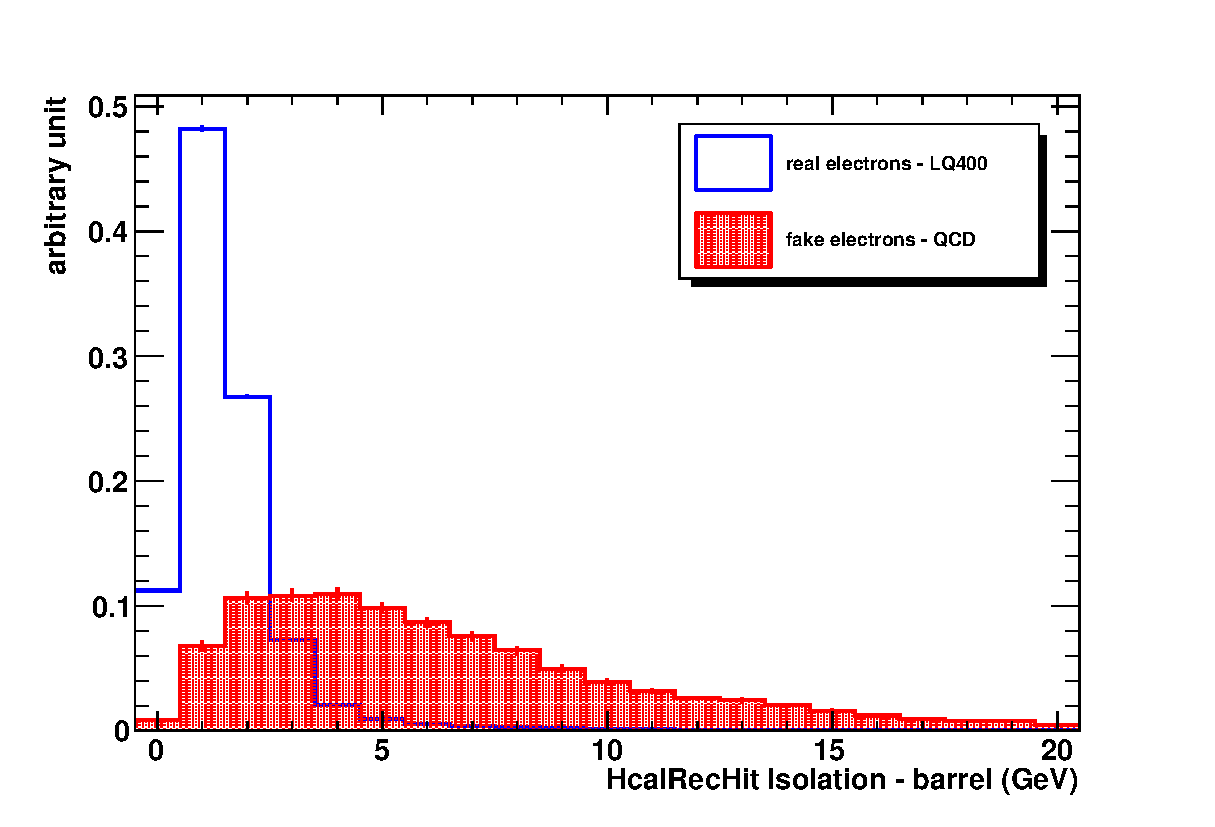
\includegraphics{plots/electronStudies/eleHcalRecHitIso_barrel_LQ400vsQCD.eps}} &
  \resizebox{7cm}{!}{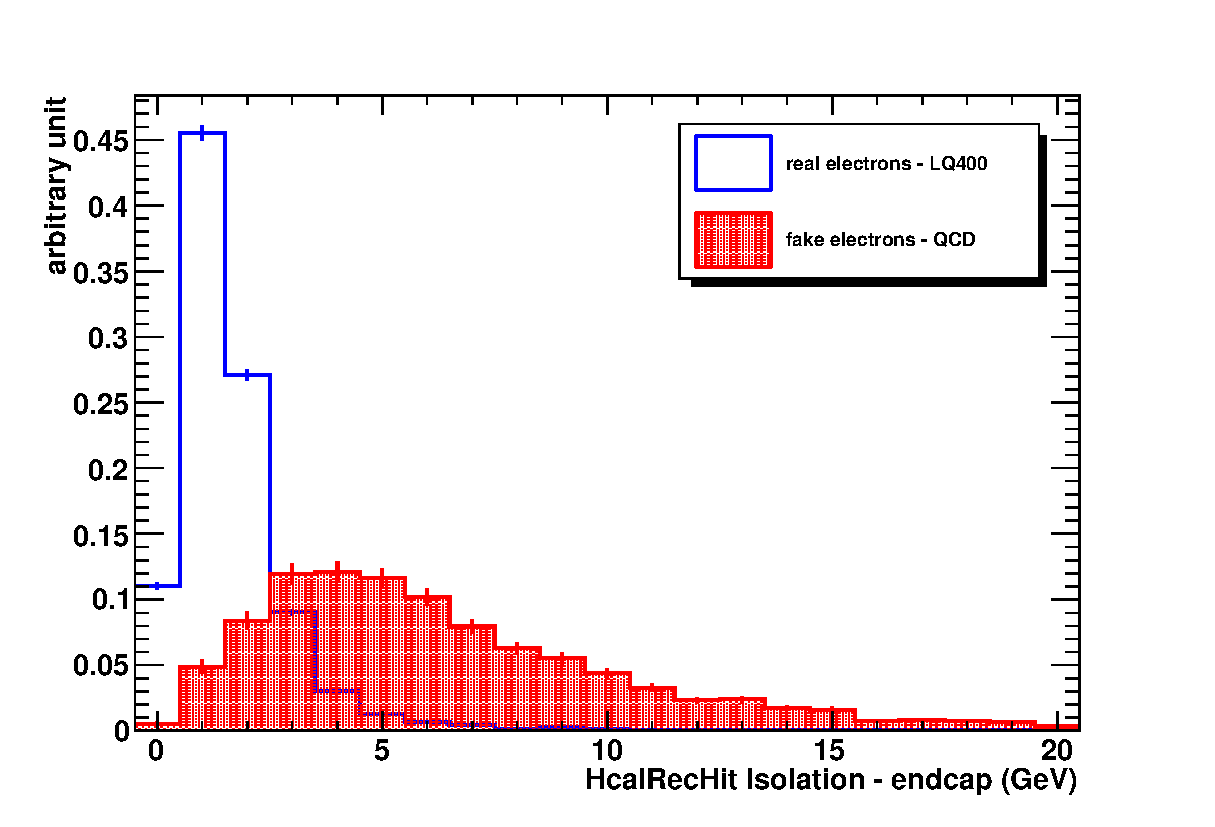
\includegraphics{plots/electronStudies/eleHcalRecHitIso_endcap_LQ400vsQCD.eps}} \\
  \resizebox{7cm}{!}{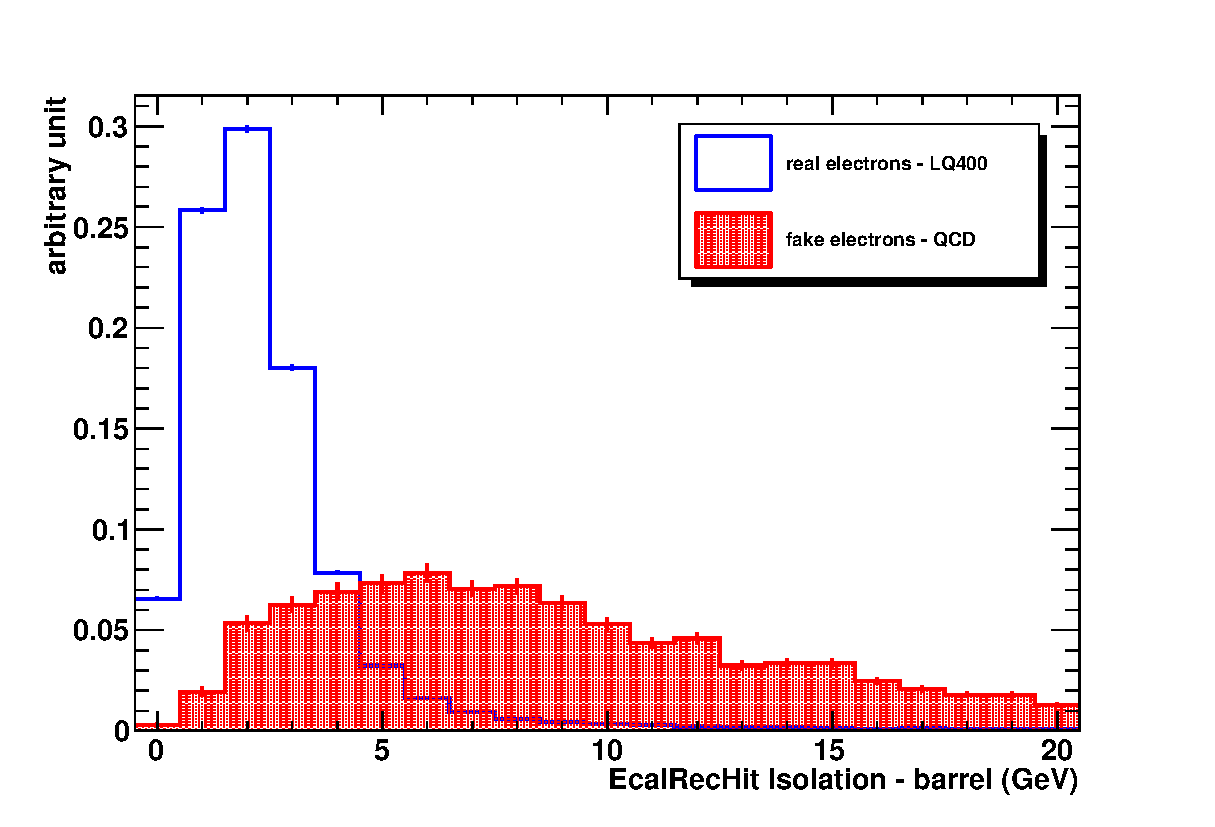
\includegraphics{plots/electronStudies/eleEcalRecHitIso_barrel_LQ400vsQCD.eps}} &
  \resizebox{7cm}{!}{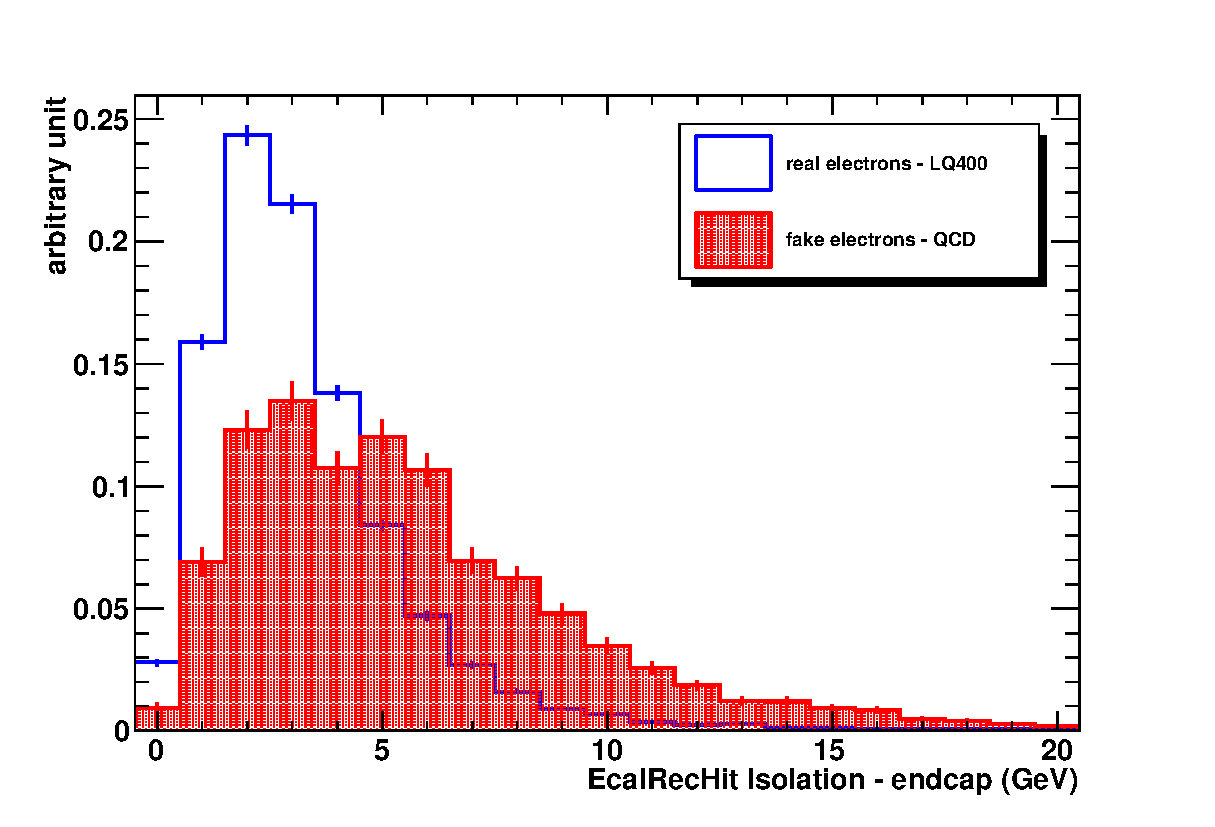
\includegraphics{plots/electronStudies/eleEcalRecHitIso_endcap_LQ400vsQCD.eps}} \\
  \end{tabular}
  \caption{\small \sl Distribution of electron-isolation variables for true electrons from the decay of LQ of mass 400 GeV, 
    and for false electrons from a sample of QCD multi jets events. Electrons with reconstructed $p_{T}>150$ GeV are made to undergo MC showed. 
    Electrons from LQ decay are matched with reconstructed electrons if $\Delta$R between them is < 0.02. FIXME}
    \label{fig:elecIso}
  \end{center}
\end{figure}

%\begin{table}[htbp]
%  \label{tab:HEEPselection}
%  \begin{center}
%    \begin{tabular}{|lcc|lcc|} \hline
%      \multicolumn{3}{lc|}{ID Variables} & \multicolumn{3}{|c|}{Isolation Variables} \\ 
%      Variable & Barrel & Endcap & Variable & Barrel & Endcap  \\ \hline
%      $H/E$  & $<0.05$ & $<0.08$ & $N_T$  & $<4$ & $<4$ \\ \hline
%      $\sigma_{\eta\eta}$  & $<0.011$ & $<0.0275$ & Track Iso (GeV) & $<7.5$ & $<15$ \\ \hline
%      $|\Delta\eta_{in}|$  & $<0.005$ & $<0.007$ & EM Iso (GeV) & $<6+0.01*E_{t}$ & $<6+0.01*E_{t}$ \\ \hline
%      $|\Delta\phi_{in}|$  & $<0.09$ & $<0.09$ & HAD Iso (GeV) & $<4+0.005*E_{t}$ & $<4+0.005*E_{t}$ \\ \hline
%    \end{tabular}
%  \caption{\small \sl HEEP electron identification and isolation criteria}
%  \end{center}
%\end{table}


\subsection{Acceptance and Reconstruction Efficiency} \label{sec:electronEfficiency}

Electrons from decays of leptoquark, 
being usually isolated from jets and having a $p_{T}$ of hundreds of GeV can be reconstructed with high efficiency. 
Table~4
%\ref{tab:ElecEffAcc} 
shows the electron acceptance in the fiducial region $A_{FR}$, the 
reconstruction efficiency within the fiducial region ($\varepsilon_{FR}^{reco}$), and the overall reconstruction efficiency 
($A_{FR} \times \varepsilon_{FR}^{reco}$) for single electrons from LQ decays for two LQ mass values.
The overall reconstruction efficiency on a single electron, including acceptance, is $= approx XX\%$ for these two LQ masses.
As an illustration, Fig \ref{fig:elecEffFV} shows the reconstruction efficiency of electrons
for LQ mass of 4000 GeV as a function of $\eta$. 
A significant loss of efficiency is seen in the region $|\eta| \approx 1.5$, and is due to the lack of calorimeter coverage between the
 ECAL barrel and the endcaps, 
a region excluded from the analyis. %INEFFICIENCY AT HIGH ETA? 

\begin{table}[htb]
  \label{tab:ElecEffAcc}
  \begin{center}
    \begin{tabular}{|l|c|c|c|} \hline
      LQ mass (GeV) & $A_{FR}$ & $\varepsilon_{FR}^{reco}$ & $A_{FR} \times \varepsilon_{FR}^{reco}$\\ \hline
      250 & 0.xx & 0.xx & 0.xx \\ \hline
      400 & 0.xx & 0.xx & 0.xx \\ \hline
    \end{tabular}
    \caption{\small \sl Electron acceptance in the fiducial region ($A_{FR}$), the 
      reconstruction efficiency within the fiducial region ($\varepsilon_{FR}^{reco}$), and the overall reconstruction efficiency 
      ($A_{FR} \times \varepsilon_{FR}^{reco}$) for single electrons from LQ decays.   Relative statistical uncertainties on overall 
      efficiency are less than 0.2.  % Is this 0.75 +- 0.02 or +- 0.015????  
      } 
  \end{center}
\end{table}

\begin{figure}
  \begin{center}
    \resizebox{9cm}{!}{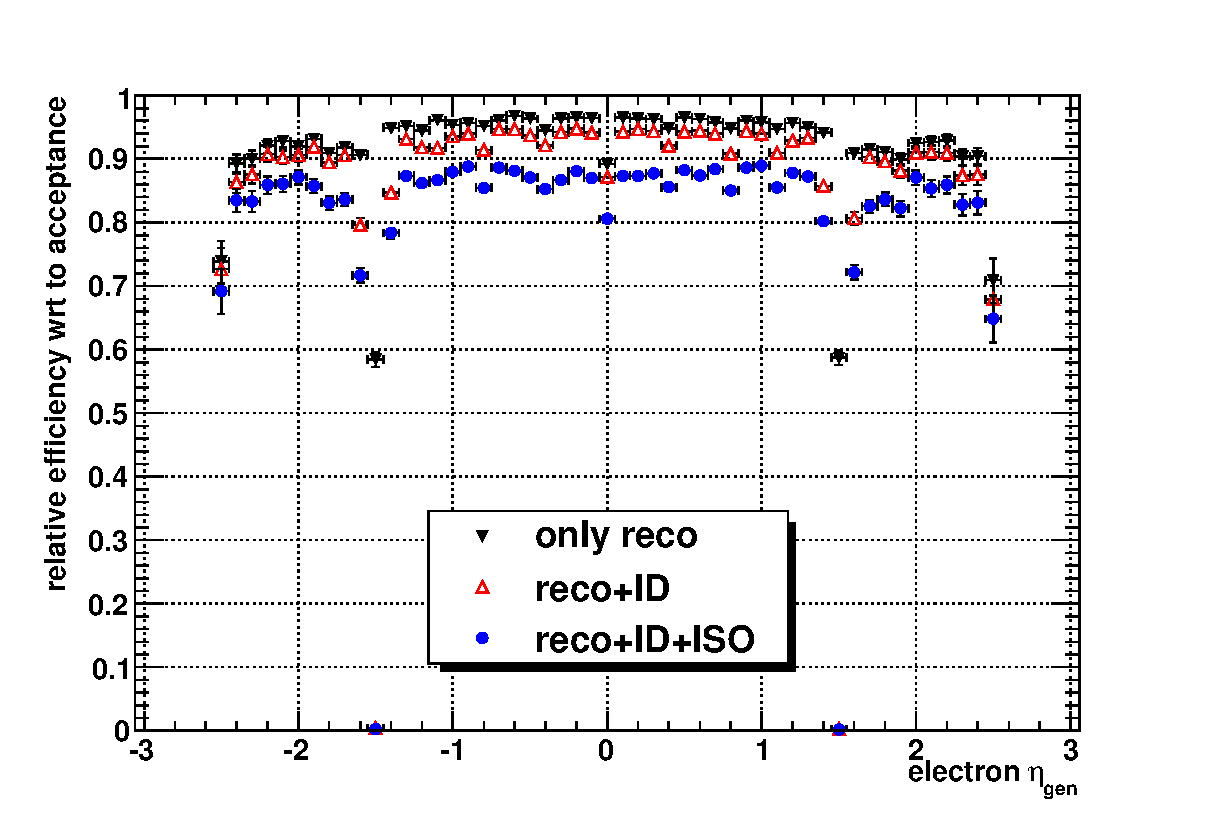
\includegraphics{plots/electronStudies/Eff_vs_Eta_recoIDIsoEle_pT30_eta2.5_LQ400.eps}}
    \caption{\small \sl Electron reconstruction efficiency as a function of $\eta$. The shaded region represents the  
      ECAL regions excluded from the fiducial volume defined at \ref{sec:IdAndIso}. The plot is for LQ mass of 400 GeV.}
    \label{fig:elecEffFV}
  \end{center}
\end{figure}

% indico.cern.ch/getFile.py/access?contribId=3&resId=0&materialId=slides&confId=32048


\begin{figure}
  \begin{center}
  \begin{tabular}{c}
    %\resizebox{9cm}{!}{\includegraphics{plots/Ele_eff_M650GeV.eps}}
    \resizebox{10cm}{!}{
\includegraphics{plots/UMD.eps}} \\
    \resizebox{10cm}{!}{
\includegraphics{plots/UMD.eps}} \\ 
%  \resizebox{5cm}{!}{
\includegraphics{plots/UMD.eps}} &
%  \resizebox{5cm}{!}{
\includegraphics{plots/UMD.eps}} \\
  \end{tabular}
  \caption{\small \sl Distributions of some reconstructed quantities for electrons from LQ decay, 
    obtained with FastSim (blue filled histogram) and FullSim (black dots) 
    samples with $M_{LQ}=650$ GeV.
    From the top-left to the bottom-right: $P_{T}$, $\eta$, $\Delta\phi_{in}$, $\Delta\eta_{in}$.}
  \label{fig:elecVariables}
  \end{center}
\end{figure}

%efficiency (pT, eta) (no deltaR from genJet since already showed distance OK above)
%pT, eta dist
%{\Large \sl Energy Resolution}
%fast vs full

%\end{document}
